\chapter{Needs Analysis and Specification}
\minitoc % Generates a mini table of contents for this chapter

\section*{Introduction}
The success of any software project depends largely on a precise understanding of user needs and the ability to translate them into concrete specifications. 
This chapter aims to define the requirements of the ERP system developed during the internship at Anter Lab. 
It begins by identifying the key actors who will interact with the system, followed by the description of functional and non-functional requirements. 
A global use case diagram is then introduced to illustrate these interactions. 
The chapter also presents a forward-looking view of the architecture, highlighting the potential shift from a monolithic MVC structure to a microservices-based design. 
Finally, the chapter concludes with the adoption of Scrum methodology for project management, detailing the backlog and sprint planning.

\section{User needs / Capturing needs}
This chapter outlines the needs analysis and specification for the ERP system developed for Anter Lab, focusing on identifying key stakeholders, defining functional and non-functional requirements, and presenting the system's use case diagram. The analysis is grounded in the high-level module overview of the ERP system, aiming to integrate essential business processes such as human resources, accounting, customer relationship management (CRM), and point-of-sale (POS) operations for small and medium-sized enterprises (SMEs).

\subsection{Identifying key players}
The ERP system involves multiple actors who interact with its various modules. Based on the system architecture and discussions with stakeholders during the internship, the primary actors are:

\begin{itemize}
    \item \textbf{Super Admin}: Has full control over the system, manages global settings, oversees all users and modules.
    \item \textbf{Admin}: Responsible for system-wide management, including authentication, user management, settings, and configuration.
    \item \textbf{Employee/User}: Engages with human resource management (HRM), project tracking, task management, and support features.
    \item \textbf{Manager}: Oversees CRM, accounting, POS, product management, and project oversight.
    \item \textbf{Client}: Interacts with project consultation, contract management, timesheets, and support services.
    \item \textbf{External Services}: APIs for third-party integrations (Zoom, Slack, Telegram, Payment gateways).
\end{itemize}

These actors were identified through a detailed analysis of the ERP module hierarchy and stakeholder feedback.

\subsection{Functional requirements}
The functional requirements specify the core functionalities the ERP system must provide, categorized by module based on the system design:

\begin{itemize}
    \item \textbf{Authentication}: Enable user login, registration, credential verification, and password reset with JWT security.
    \item \textbf{HRM Management}: Manage employee appraisals, recruitment, onboarding, attendance, leave, payroll, and collaboration events.
    \item \textbf{Accounting Management}: Handle purchasing, expenses, sales, budgeting, planning, and core accounting tasks.
    \item \textbf{CRM Management}: Support lead lifecycle management, deal pipelines, contract handling, feedback collection, and CRM configuration.
    \item \textbf{Project Management}: Facilitate project tracking, task assignment, and timesheet management.
    \item \textbf{User Management}: Provide user account creation, role assignment, permissions, and notifications.
    \item \textbf{Product Management}: Track product stock, manage pricing, and control warehouse and inventory.
    \item \textbf{POS Management}: Manage quotations, POS transactions, purchases, and transfer operations.
    \item \textbf{Support Management}: Integrate communication tools like Zoom, Telegram, Chat, and Slack for support services.
    \item \textbf{Settings Management}: Allow configuration of login settings and general system parameters.
    \item \textbf{Client Features}: Enable clients to consult projects, contracts, timesheets, calendars, tasks, bugs, and support requests.
    \item \textbf{Notification System}: Send real-time alerts for HR, accounting, CRM, or system activities.
    \item \textbf{Audit Logging}: Track all system actions for compliance and debugging.
    \item \textbf{Reporting \& Analytics}: Generate reports for HRM, Accounting, CRM, and POS modules.
    \item \textbf{Integration Layer}: Allow external APIs (e.g., payment gateways) to communicate with the ERP.
\end{itemize}

These requirements ensure comprehensive coverage of SME business processes.

\subsection{Non-functional requirements}
The non-functional requirements define the system's quality attributes to ensure reliability and usability:

\begin{itemize}
    \item \textbf{Security}: Implement JWT authentication to secure all API endpoints and protect sensitive data.
    \item \textbf{Performance}: Ensure API responses within 2 seconds under typical load, with optimized MySQL queries.
    \item \textbf{Scalability}: Support up to 100 concurrent users, with a modular design for future growth.
    \item \textbf{Usability}: Provide intuitive APIs with Postman documentation, supporting web and mobile interfaces.
    \item \textbf{Reliability}: Achieve 99\% uptime with robust error handling and logging in Laravel.
    \item \textbf{Maintainability}: Adhere to MVC architecture for easy updates, using Git for version control.
    \item \textbf{Auditability}: Keep secure logs of critical operations for compliance.
    \item \textbf{Data Backup \& Recovery}: Ensure automatic daily backups and quick recovery procedures.
    \item \textbf{Continuous Integration/Delivery (CI/CD)}: Use GitLab pipelines for automated testing and deployment.
\end{itemize}

These attributes guarantee a robust and adaptable system.

\subsection{Overall Use Case Diagram}
The overall use case diagram illustrates the interactions between actors and the ERP system's functionalities. This diagram is derived from the module hierarchy and functional requirements outlined above.

\begin{figure}[H]
    \centering
    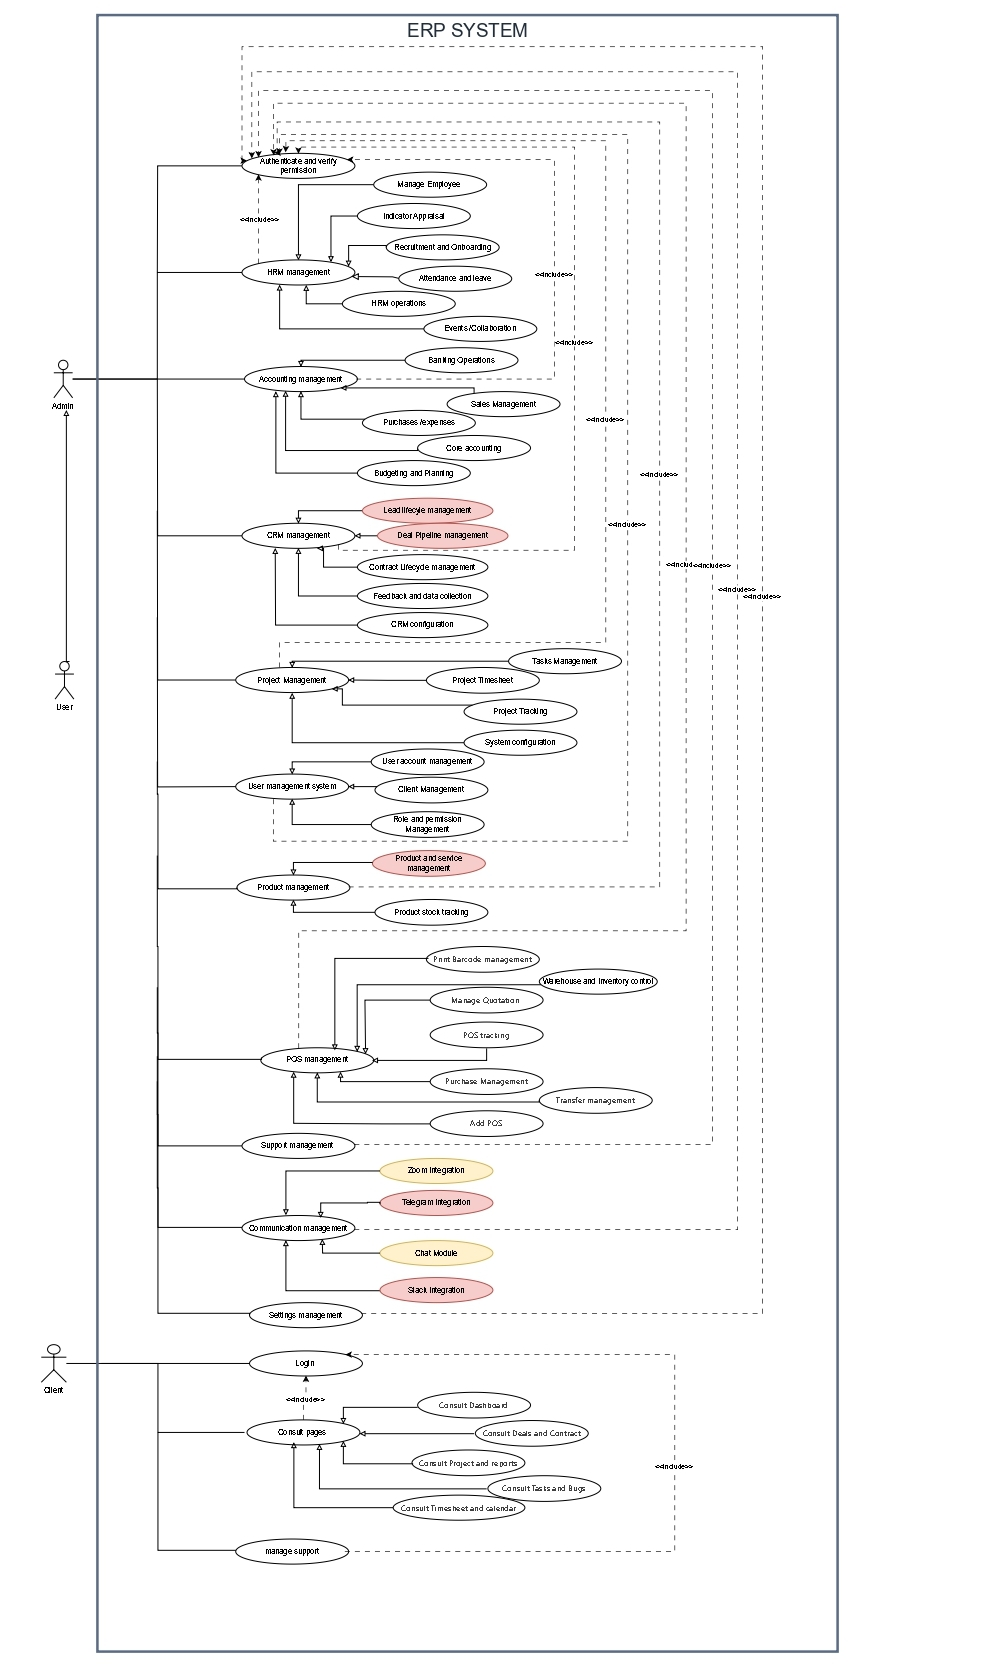
\includegraphics[width=0.9\textwidth]{chapters/chapter 2/figures/diagramGeneralUseCase (1) (1).drawio (1)_page-0001 (1).jpg}
    \caption{Overall Use Case Diagram of the ERP System}
    \label{fig:overall_use_case}
\end{figure}

\subsection{Micro-services Architecture}
While the current implementation follows a monolithic MVC architecture using Laravel, a future transition to a microservices architecture is considered for enhanced scalability. Each module (e.g., HRM, CRM, POS) could operate as an independent service, communicating via REST APIs.

\begin{figure}[H]
    \centering
    \begin{tikzpicture}[
        node distance=1.5cm and 2cm,
        service/.style={
            draw, 
            rectangle, 
            rounded corners=4pt,
            minimum width=3cm, 
            minimum height=1.5cm,
            align=center,
            text width=2.8cm,
            font=\small,
            fill=green!10
        },
        gateway/.style={
            service,
            fill=blue!10,
            minimum width=4cm
        },
        db/.style={
            service,
            fill=gray!10,
            minimum height=2cm
        },
        arrow/.style={
            ->,
            thick,
            shorten >=2pt,
            shorten <=2pt
        }
    ]
        % API Gateway (Central Hub)
        \node[gateway] (api_gateway) {API Gateway};
        
        % Microservices
        \node[service, below=of api_gateway, xshift=-4cm] (auth_service) {Authentication Service};
        \node[service, below=of api_gateway] (hrm_service) {HRM Service};
        \node[service, below=of api_gateway, xshift=4cm] (crm_service) {CRM Service};
        \node[service, below=of hrm_service, xshift=-4cm] (pos_service) {POS Service};
        \node[service, below=of hrm_service] (accounting_service) {Accounting Service};
        \node[service, below=of hrm_service, xshift=4cm] (user_service) {User Management Service};
        \node[service, below=of accounting_service, xshift=-2cm] (product_service) {Product Management Service};
        \node[service, below=of accounting_service, xshift=2cm] (support_service) {Support Service};
        
        % Database Layer
        \node[db, below=of support_service, xshift=0cm] (database) {Central Database (MySQL)};
        
        % Arrows from Gateway to Services
        \draw[arrow] (api_gateway) -- (auth_service);
        \draw[arrow] (api_gateway) -- (hrm_service);
        \draw[arrow] (api_gateway) -- (crm_service);
        \draw[arrow] (api_gateway) -| (pos_service);
        \draw[arrow] (api_gateway) -| (accounting_service);
        \draw[arrow] (api_gateway) -| (user_service);
        \draw[arrow] (api_gateway) -| (product_service);
        \draw[arrow] (api_gateway) -| (support_service);
        
        % Arrows from Services to Database
        \draw[arrow] (auth_service) -- (database);
        \draw[arrow] (hrm_service) -- (database);
        \draw[arrow] (crm_service) -- (database);
        \draw[arrow] (pos_service) -- (database);
        \draw[arrow] (accounting_service) -- (database);
        \draw[arrow] (user_service) -- (database);
        \draw[arrow] (product_service) -- (database);
        \draw[arrow] (support_service) -- (database);
    \end{tikzpicture}
    \caption{Microservices Architecture Overview}
    \label{fig:microservices}
\end{figure}

\section{Project management with Scrum}
The development process adopts the Scrum methodology to manage iterative progress, ensuring flexibility and regular feedback.

\subsection{Product backlog}
The product backlog contains prioritized user stories to guide sprint planning:

\begin{longtable}{|p{3cm}|p{5cm}|p{3cm}|p{2cm}|}
\hline
\textbf{User Story} & \textbf{Description} & \textbf{Priority} & \textbf{Estimate} \\
\hline
\endfirsthead
\hline
\textbf{User Story} & \textbf{Description} & \textbf{Priority} & \textbf{Estimate} \\
\hline
\endhead
As a Super Admin, I want to configure system-wide parameters. & Manage ERP modules, integrations, and roles globally. & High & 8 \\
\hline
As an Admin, I want to authenticate users with JWT. & Implement secure login, registration, and verification. & High & 5 \\
\hline
As a Manager, I want to manage HRM functions. & CRUD for appraisals, recruitment, attendance. & High & 8 \\
\hline
As a Manager, I want to handle accounting tasks. & Manage purchases, sales, budgeting. & Medium & 7 \\
\hline
As a Manager, I want to manage CRM leads. & Lead lifecycle, deal pipelines, contracts. & Medium & 6 \\
\hline
As an Employee, I want to track projects. & Task assignment, timesheets, tracking. & High & 5 \\
\hline
As an Admin, I want to manage user accounts. & Role assignment, permissions, notifications. & High & 4 \\
\hline
As a Manager, I want to manage products. & Stock, pricing, inventory control. & Medium & 6 \\
\hline
As a Manager, I want to handle POS operations. & Quotations, purchases, transfers. & Medium & 5 \\
\hline
As an Employee, I want support integrations. & Zoom, Telegram, Chat, Slack. & Low & 3 \\
\hline
As a Client, I want to consult project details. & View projects, contracts, timesheets. & Medium & 4 \\
\hline
As an Admin, I want to see system audit logs. & Track sensitive actions for compliance. & High & 6 \\
\hline
As a Manager, I want reporting dashboards. & Generate HR, CRM, Accounting KPIs. & Medium & 7 \\
\hline
As a Developer, I want CI/CD pipelines. & Automate testing and deployment with GitLab. & High & 5 \\
\hline
\caption{Product Backlog}
\label{tab:product_backlog}
\end{longtable}

\subsection{Sprint Planning}
The internship project was organized using the \textbf{Scrum framework}, with weekly sprints due to the one-month duration. Each sprint was carefully planned with specific objectives to ensure steady progress and incremental delivery.

\begin{longtable}{|p{1.5cm}|p{4cm}|p{2.5cm}|p{5.5cm}|}
\hline
\textbf{Sprint} & \textbf{Objective} & \textbf{Duration} & \textbf{Main Tasks (Planned)} \\
\hline
\endfirsthead
\hline
\textbf{Sprint} & \textbf{Objective} & \textbf{Duration} & \textbf{Main Tasks (Planned)} \\
\hline
\endhead
\textbf{Sprint 0} & Project setup and team onboarding & Week 1 & 
\begin{itemize}
    \item Clone and run project locally from GitLab
    \item Configure database and run migrations
    \item Join ClickUp workspace and Discord server
    \item Setup backend foundation (API scaffolding)
    \item Implement initial APIs: Register, Login, getUserInfo
    \item Migrate Dashboard Controller to API version
\end{itemize} \\
\hline
\textbf{Sprint 1} & Core administrative APIs & Week 2 & 
\begin{itemize}
    \item CRUD operations for Employees (with Import/Export)
    \item CRUD operations for Branches
    \item CRUD operations for Departments
    \item CRUD operations for Designations
\end{itemize} \\
\hline
\textbf{Sprint 2} & Configuration \& Option Management APIs & Week 3 & 
\begin{itemize}
    \item Leave Type, Document Type, Payslip Type APIs
    \item Allowance Option, Loan Option, Deduction Option APIs
    \item Goal Type, Training Type, Award Type APIs
    \item Termination Type, Job Category, Job Stage APIs
    \item Performance Type, Competencies APIs
\end{itemize} \\
\hline
\textbf{Sprint 3} & Reporting \& Data Export APIs & Week 4 & 
\begin{itemize}
    \item Financial Summary Reports: Income, Expense, Cash Flow, Tax
    \item Transaction Reports: Invoices, Sales, Purchases, Receivables/Payables
    \item Inventory, Ledger, and Account Statement reports
    \item Data Export APIs for all reports
\end{itemize} \\
\hline
\caption{Sprint Planning Overview}
\label{tab:sprint_planning}
\end{longtable}

\section*{Conclusion}
In summary, this chapter established a solid foundation for the ERP system by identifying stakeholders, capturing functional and non-functional requirements, and illustrating the interactions through use case diagrams. 
The analysis highlighted not only the core modules (HRM, Accounting, CRM, POS, etc.) but also additional cross-cutting concerns such as authentication, reporting, and integration with external services. 
Furthermore, non-functional requirements such as security, scalability, and maintainability were emphasized to ensure the system’s robustness. 
The sprint planning section provided a roadmap for iterative development using the Scrum framework, ensuring that progress could be tracked weekly and objectives refined based on feedback. 
This detailed specification phase paves the way for the implementation stage, which will be covered in Chapter 3, focusing on the execution of each sprint.